\section{Processi organizzativi}
\label{processiorganizzativi}

\subsection{Processo di gestione del progetto}
\label{gestioneprogetto}
Il processo di gestione del progetto contiene tutte le attività ed i compiti che consentono la gestione del processo di sviluppo (vedi sezione \ref{processosviluppo}). Il \projectManager{} avrà il compito di pianificare le varie attività, gestire le risorse ed Analizzare e prevenire i rischi.\\
Il processo di gestione del progetto è composto dalle seguenti attività:
\begin{itemize}
\item \textbf{Pianificazione;}
\item \textbf{Esecuzione e controllo;}
\end{itemize}

\subsubsection{Pianificazione}
\label{pianificazione}
Lo scopo di quest'attività è di preparare un piano di esecuzione del processo. Il \projectManager{} ha il compito di redigere tale piano e di produrre la relativa documentazione (vedi paragrafi relativi al \textit{Piano di Progetto} nelle sezioni \ref{pianificazionedocumenti} e \ref{progettazionesviluppo}).

\paragraph{\underline{Pianificare attività}:} per pianificare le varie attività da svolgere, il \projectManager{} dovrà utilizzare gli strumenti identificati nel paragrafo dedicato ai diagrammi di Gantt\g{} nella sezione \ref{definizioneinfrastruttura}. Tali diagrammi dovranno essere inclusi nella documentazione.

\paragraph{\underline{Gestione delle risorse}:} per gestire le varie risorse disponibili durante lo svolgimento del progetto, il \projectManager{} dovrà creare dei diagrammi delle risorse, per pianificare la quantità di ore che ogni risorsa dovrà dedicare a ciascuna attività. Per disegnare i diagrammi di attività, si dovranno utilizzare gli strumenti identificati nel paragrafo dedicato ai diagrammi di Gantt\g{} nella sezione \ref{definizioneinfrastruttura}. Tali diagrammi dovranno essere inclusi nella documentazione.
Inoltre, per assegnare i compiti alle risorse disponibili, il \projectManager{} utilizzerà il sistema di ticketing offerto da GitHub\g{}\footnote{Per maggiori informazioni consultare la sezione \ref{github}.}.

\subparagraph{Rotazione dei ruoli:} durante lo svolgimento del progetto, è necessario che tutti i componenti del gruppo ricoprano tutti i vari ruoli definiti nel \PdP{}. Nel precedente documento verranno inoltre specificate le assegnazioni dei ruoli alle risorse, ripartite temporalmente e il quantitativo di ore che ciascuna risorsa dovrà svolgere in veste di un determinato ruolo.\\
Per pianificare l'impiego delle risorse in tale senso, il \projectManager{} si ispirerà alle seguenti regole:
\begin{itemize}
	\item Ogni risorsa dovrà ricoprire tutti i ruoli;
	\item Il carico di ore individuali dovrà essere equo.
\end{itemize}
Riportiamo di seguito le direttive che regolano l'assegnazione e la modalità di rotazione dei ruoli.\\
I ruoli verranno assegnati alle risorse in modo tale che cambino al termine di una macro-fase (vedi \PdP). Dato che i ruoli da ricoprire sono in quantità minore rispetto alle risorse, sarà necessario che una o più risorse ricoprano più ruoli durante la stessa macro-fase. Per regolamentare questa ulteriore rotazione, le risorse ricopriranno un singolo ruolo per settimana, ruotando tra i ruoli assegnati nella specifica macro-fase.\\
Ogni componente del gruppo potrà consultare, in qualsiasi momento, i diagrammi di Gantt\glossario{} che descrivono la gestione delle risorse e dei ruoli, in maniera tale che ognuno potrà sempre essere consapevole del ruolo ricoperto dagli altri componenti.

\paragraph{\underline{Analisi e prevenzione dei rischi}:} durante l'intero periodo di svolgimento del progetto, il \projectManager{} dovrà analizzare i rischi che possono incombere. Inoltre dovrà cercare di prevenirli e trovare delle contromisure ad essi. Tale analisi dovrà essere inclusa nella relativa documentazione.

\subsubsection{Esecuzione e controllo}
\label{esecuzionecontrollo}

\paragraph{\underline{Incontri}:} sarà il \projectManager{} a fissare gli incontri, sia interni che esterni.
\\Per ogni incontro dovrà essere specificata data, ora, luogo, ordine del giorno e motivi della riunione; tali informazioni dovranno essere rese disponibili con almeno quattro giorni di anticipo.
\\Successivamente alla decisione di una nuova data il \projectManager{} provvederà alla creazione di un evento sul calendario condiviso su Google Calendar\glossario{}.

\subparagraph{Incontri esterni:} sarà il \projectManager{} a fissare gli incontri con i proponenti e/o committenti utilizzando la casella di posta creata appositamente\footnote{Si veda il paragrafo \textit{Strumenti di comunicazione} della sezione \ref{definizioneinfrastruttura}}.
Il \projectManager{} prima di prendere alcun accordo con le parti esterne dovrà contattare i vari componenti del gruppo, per sentire se almeno cinque membri concordano.
\\In caso positivo il \projectManager{} provvederà a contattare i proponenti e/o committenti per fissare la data dell'incontro.
\\Sarà compito del \projectManager{} redigere il verbale dell'incontro avvenuto.

\subparagraph{Incontri interni:} sarà il \projectManager{} a fissare gli incontri interni, contattando tutti i membri del gruppo. Gli incontri interni dovranno avere una frequenza almeno quindicinale.
Ogni componente del gruppo è tenuto a leggere regolarmente la posta elettronica personale e rispondere ad eventuali richieste di un incontro interno.
Nel caso in cui i membri disponibili a partecipare alla riunione in una certa data siano meno di quattro, questa verrà posticipata o anticipata, in modo che siano presenti un numero adeguato di persone.
Inoltre, è possibile e auspicabile che siano necessarie riunioni tra specifici membri del gruppo, ad esempio: in fase di analisi può essere utile che solo gli \emph{Analisti} si incontrino tra di loro, senza il resto del gruppo.
I restanti componenti del gruppo saranno comunque informati sui contenuti e le decisioni prese tramite invio di una e-mail alla mailing list\glossario{} o alla pubblicazione di un verbale sul repository\glossario{} nel caso siano state prese decisioni importanti.
\subparagraph{Richieste di incontri:} qualora ve ne sia la necessità, ogni membro del gruppo potrà richiedere un incontro sia interno che esterno, contattando personalmente il \projectManager{} ed esponendo i motivi della richiesta.
\\Il \projectManager{} avrà potere di scegliere se accettare o rifiutare la richiesta.

\paragraph{\underline{Creazione milestone}:} il \projectManager{} dovrà provvedere alla creazione di una milestone\g{} per la prossima revisione a cui il gruppo \authorName{} ha intenzione di partecipare. La gestione di una milestone\g{} prevede l'apertura di una serie di ticket, atti a pianificare i compiti da svolgere entro la chiusura della stessa (vedi figura \ref{gestione_milestone}).\\
Per la procedura di apertura di una milestone si veda il paragrafo \textit{Creazione milestone} in sezione \ref{proceduregithub}.
\begin{figure}[!h]
	\centering
	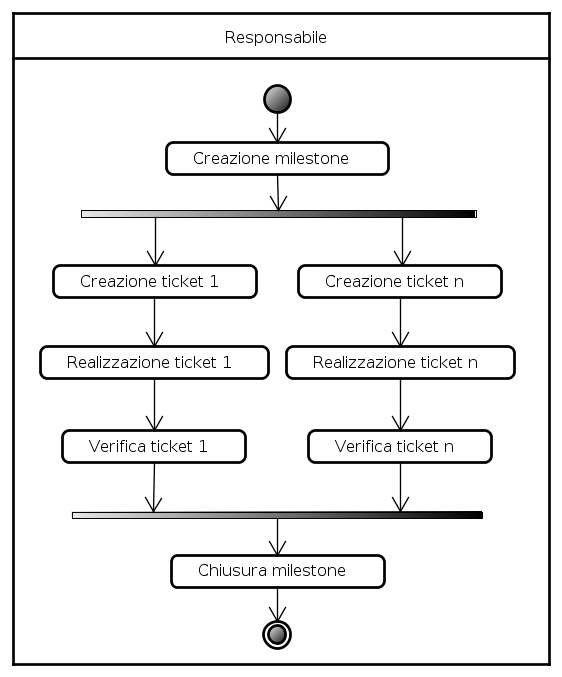
\includegraphics[scale=0.5]{./content/Immagini/Avanzamento_Milestone.png}
	\caption{Modello per la gestione di una milestone}
	\label{gestione_milestone}
\end{figure}

\paragraph{\underline{Creazione ticket}:} i ticket vengono creati da:
\begin{itemize}
\item \textbf{Responsabile di Progetto:} crea la maggioranza dei ticket;
\item \textbf{Verificatore:} crea i ticket per segnalare le imprecisioni o errori trovati durante la verifica.
\end{itemize}
Ogni ticket dovrà essere assegnato ad un unico membro del team \authorName{} e dovrà avere le seguenti caratteristiche\footnote{In figura 3 è mostrata l'interfaccia per la creazione di ticket.}:
\begin{itemize}
\item{\textbf{Destinatario:}} a chi è rivolto l'attività indicata dal ticket;
\item{\textbf{Milestone:}} la milestone\glossario{} a cui è associato il ticket;
\item{\textbf{File:}} dovrà essere indicato il file oggetto dell'attività;
\item{\textbf{Label:}} ogni ticket avrà una o più label associate; le label possibili sono le seguenti:
\begin{itemize}
\item\textbf{Modifica:} ticket generalmente creato dal \emph{Verificatore} per segnalare gli errori trovati;
\item\textbf{Verifica:} ticket creato dal \projectManager{} per assegnare la verifica a uno dei \emph{Verificatori};
\item\textbf{Richiesta approvazione:} ticket creato da un \emph{Verificatore} per richiedere l'approvazione di un documento;
\item\textbf{Creazione:} ticket creato dal \projectManager{} per assegnare un compito a un generico membro del gruppo;
\item\textbf{Priorità alta:} label assegnata ad un ticket creato per la gestione di anomalie;
\item\textbf{Priorità media:} label assegnata ad un ticket creato per la gestione di discrepanze di media gravità;
\item\textbf{Priorità bassa:} label assegnata ad un ticket creato per la gestione di discrepanze non gravi.
\end{itemize}
\end{itemize}
Si vedano le figure \ref{creazione_ticketstd} e \ref{creazione_ticketver}, per i diagrammi di attività della gestione dei ticket. Per la procedura di apertura di un ticket, si veda il paragrafo \textit{Creazione ticket} nella sezione \ref{proceduregithub}.
\begin{figure}[h!]
	\centering
	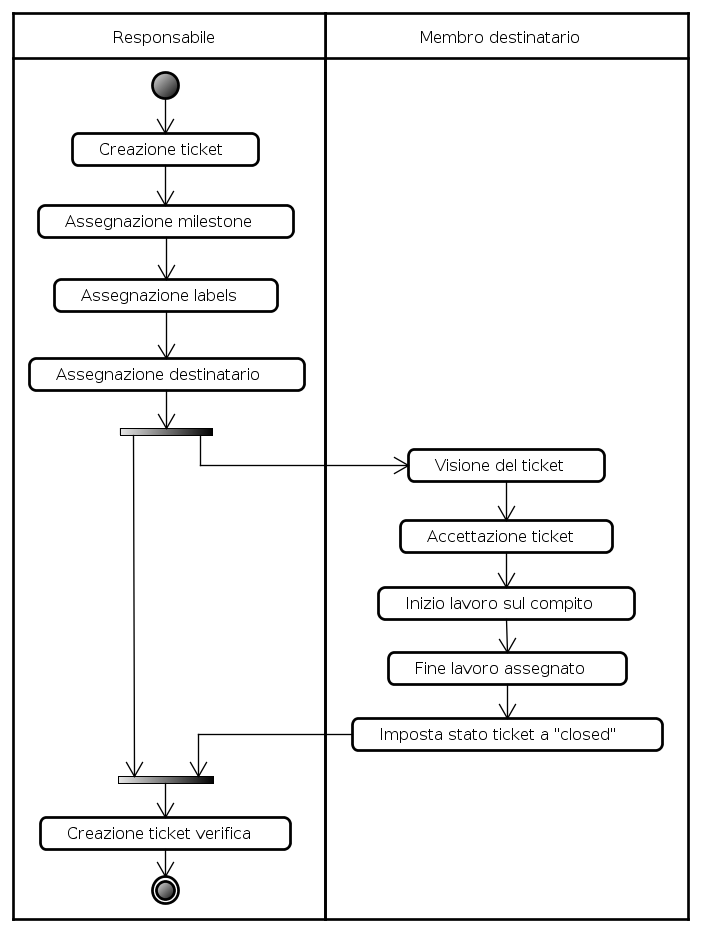
\includegraphics[scale=0.5]{./content/Immagini/Creazione_Compito}
	\caption{Modello di ticket per la creazione di un compito generico}
	\label{creazione_ticketstd}
\end{figure}

\begin{figure}[h!]
	\centering
	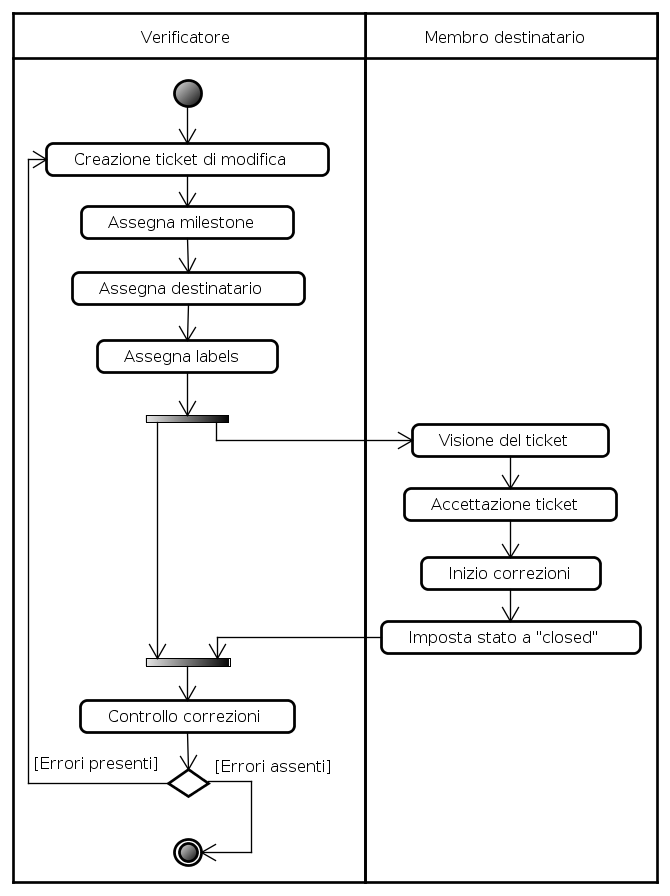
\includegraphics[scale=0.5]{./content/Immagini/Ticket_Verificato}
	\caption{Modello di ticket per la creazione di un ticket di verifica}
	\label{creazione_ticketver}
\end{figure}

\paragraph{\underline{Esecuzione dei compiti}:} ogni membro del gruppo dovrà visionare i ticket a lui assegnati e, successivamente all'esecuzione del compito, dovrà cambiare lo stato del ticket in \lq\lq{}closed\rq\rq{}. Quando il destinatario del ticket ne prenderà visione, dovrà confermarlo con un commento nella pagina web del ticket. Se il \projectManager{} si rende conto che un ticket non è stato eseguito come atteso, \lq\lq{}riaprirà\rq\rq{} il ticket.

\paragraph{\underline{Chiusura milestone}:} nel momento in cui tutti i ticket riferiti ad una milestone\g{} sono stati completati e chiusi, sarà cura del \projectManager{} verificarne l'effettiva chiusura e di conseguenza chiudere la milestone\g{}. Si veda il paragrafo \textit{Chiusura milestone} della sezione \ref{proceduregithub} per la relativa procedura.

\subsection{Processo di organizzazione dell'infrastruttura}
\label{organizzazioneinfrastruttura}
Il processo di organizzazione dell'infrastruttura consente di fornire servizi ed infrastrutture operative in grado di supportare le esigenze dei processi che il gruppo \authorName{} intende implementare durante tutto il ciclo di vita del software. Questo processo definisce, fornisce e mantiene i mezzi e le tecnologie chiave di cui ha bisogno il team per lo svolgimento delle proprie attività.\\
Il processo di organizzazione dell'infrastruttura è composto dalle seguenti attività:
\begin{itemize}
\item \textbf{Definizione dell'infrastruttura;}
\end{itemize}

\subsubsection{Definizione dell'infrastruttura}
\label{definizioneinfrastruttura}
Lo scopo di quest'attività è di individuare quali infrastrutture sono necessarie per lo svolgimento dei vari processi. Nei seguenti paragrafi verranno definiti gli strumenti, individuati dagli \textit{Amministratori}, di cui il team necessita per lo svolgimento di un progetto. Ogni strumento dovrà essere documentato per quanto riguarda l'installazione e l'esecuzione delle procedure ricorrenti (vedi \ref{strumenti}).

\paragraph{\underline{Ambiente di sviluppo}:} il sistema operativo utilizzato per lo sviluppo del progetto è a discrezione di ogni singolo componente del gruppo. I vari membri del gruppo utilizzeranno i seguenti sistemi operativi:
\begin{itemize}
\item Ubuntu 12.04 64bit;
\item Mac OS\g{} 10.9 64bit;
\item Windows\g{} 8 64bit.
\end{itemize}

\paragraph{\underline{Controllo di versione}:} è necessario usufruire di un controllo di versione per lo sviluppo della documentazione e del codice. Per questo verranno creati due repository\g{} distinti. Essi saranno privati e quindi accessibili solo ai membri del team.\\
I repository\g{} saranno ospitati dal servizio GitHub\g{}, il quale utilizza il sistema di versionamento Git\g{}. Per quanto riguarda le procedure di interazione e di installazione, vedere il paragrafo \ref{git}.

\subparagraph{Repository della documentazione:}
\label{rdocumentazione}
all'interno di questo repository\g{} verranno memorizzati tutti i file necessari alla generazione dei documenti. Di seguito verrà descritta sinteticamente l'organizzazione interna del filesystem.

\begin{figure}[h!]
\centering
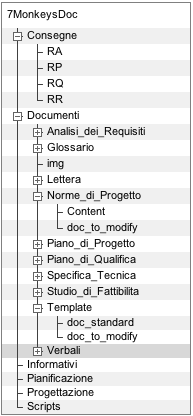
\includegraphics[scale=0.5]{./content/Immagini/Filesystem}
\caption{Organizzazione file system del repository dei documenti.}
\label{filesystem}
\end{figure}

\begin{itemize}
\item\textbf{Consegne:} contiene tutti i documenti in formato \verb!PDF!\glossario{} consegnati nelle varie revisioni. I file sono raggruppati in sotto cartelle denominate con l'acronimo della revisione a cui fanno riferimento. La struttura delle sottocartelle sarà la seguente:
\begin{itemize}
\item\textbf{RR:} Revisione dei Requisiti;
\item\textbf{RP:} Revisione di Progettazione;
\item\textbf{RQ:} Revisione di Qualifica;
\item\textbf{RA:} Revisione di Accettazione.
\end{itemize}

\item\textbf{Documenti:} è la cartella contenente i sorgenti di tutti i documenti, sia in stato di redazione, sia completati. Il suo contenuto è organizzato nel seguente modo:
\begin{itemize}
\item\textbf{Nome\_del\_Documento:} ogni documento in fase di redazione dovrà avere la propria cartella, denominata con lo stesso nome del documento (vedi \ref{filesystem}). Se il documento necessità di immagini, esse dovranno essere salvate in una sottocartella denominata \lq\lq{}Immagini\rq\rq{};
\item \textbf{Template:} contiene i template \LaTeX{} comuni a tutti i documenti necessari per la loro compilazione. In particolare, in essi vengono definiti gli stili delle pagine, il frontespizio e i vari comandi creati per la stesura;
\item \textbf{Verbali:} contiene i verbali redatti dal gruppo durante lo svolgimento del progetto. Per ogni documento verrà creata una sottocartella apposita, contenente i file necessari.
\end{itemize}

\item\textbf{Informativi:} contiene dei file informativi; per esempio è presente una procedura per la creazione di un nuovo documento e un file contenente la lista di tutti i comandi \LaTeX utilizzati nei file di compilazione;

\item\textbf{Pianificazione:} contiene tutti i grafici Gantt\g{} utilizzati nella pianificazione delle attività e nella gestione delle risorse;

\item\textbf{Progettazione:} contiene tutti i diagrammi UML\g{} utilizzati durante la progettazione del software;
\item\textbf{Scripts:} contiene gli script utilizzati per automatizzare alcune procedure; per esempio la compilazione dei documenti per una consegna.
\end{itemize}

\subparagraph{Repository del codice:}
\label{repocodice}
all'interno di questo repository\g{} verranno memorizzato il codice sorgente del software e la relativa documentazione. Di seguito verrà descritta sinteticamente l'organizzazione interna del filesystem.

\begin{figure}[h!]
\centering
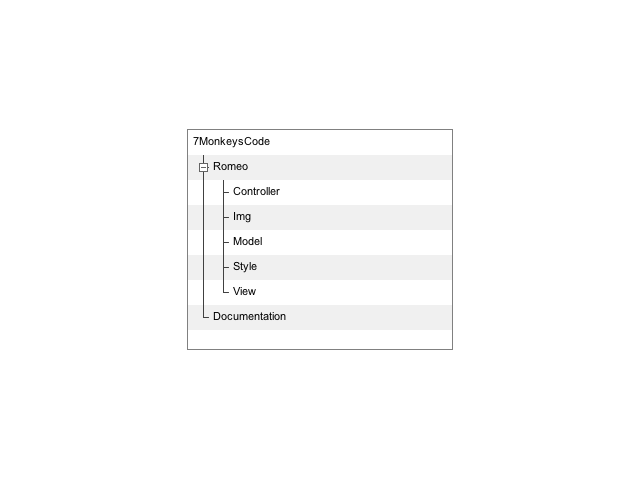
\includegraphics[scale=0.5]{./content/Immagini/filesystemcode}
\caption{Organizzazione file system del repository del codice.}
\label{filesystemcodice}
\end{figure}

\begin{itemize}
\item \textbf{Romeo:} è la cartella principale, contenente i sorgenti dell'applicativo \project{}. Il suo contenuto è organizzato come segue:
\begin{itemize}
\item \textbf{Controller:} contiene il codice relativo al componente \textit{Controller} dell'architettura software;
\item \textbf{Img:} contiene le immagini che faranno parte della GUI\g{} del software;
\item \textbf{Model:} contiene il codice relativo al componente \textit{Model} dell'architettura software;
\item \textbf{Style:} contiene i fogli di stile relativi alle finestre dell'applicativo;
\item \textbf{View:} contiene il codice relativo al componente \textit{View} dell'architettura software.
\end{itemize}
\item \textbf{Documentation:} contiene i file di documentazione, generati dalla compilazione del codice sorgente.
\end{itemize}

\paragraph{\underline{Stesura documentazione}:} è necessario utilizzare un sistema di stesura dei documenti che venga incontro alle esigenze tipografiche, di personalizzazione e che inoltre permetta il controllo di versione dei file. Conseguentemente, potrà essere individuato un editor testuale adeguato alle esigenze di sviluppo.\\
Verrà quindi utilizzato il linguaggio di markup\g{} \LaTeX{} (vedi sezione \ref{latex}) e l'editor \textit{TexMaker}  (vedi sezione \ref{texmaker}).

\paragraph{\underline{Diagrammi UML}:} è necessario individuare gli strumenti adatti per la produzione dei grafici UML\g{} che saranno inseriti nella documentazione. Tali diagrammi dovranno essere conformi allo standard UML\g{} 2.0.\\
Verranno quindi utilizzati: \textit{Astah}\g{} - \textit{Professional Edition} per la produzione dei diagrammi dei casi d'uso e di attività (vedi sezione \ref{astah}) e \textit{Visual Paradigm} per i diagrammi di package e di classe (vedi sezione \ref{visualparadigm}). 

\paragraph{\underline{Diagrammi di Gantt}:} è necessario individuare gli strumenti adatti per pianificare la gestione di progetto e gestire le risorse umane. In particolare, sarà necessario produrre dei diagrammi di Gantt\g{} che andranno inseriti nella documentazione.\\
Verrà quindi utilizzato \textit{GanttProject}\g{} (vedi sezione \ref{ganttproject}).

\paragraph{\underline{Codifica}:} è necessario individuare gli strumenti adatti per la codifica del codice. Gli strumenti possono comprendere:
\begin{itemize}
\item \textbf{Librerie esterne:} eventualmente individuate durante la progettazione architetturale (vedi \ref{progarchitetturale});
\item \textbf{Framework:} costituiscono eventualmente la base su cui sviluppare il prodotto, da individuare in base alle esigenze di progettazione;
\item \textbf{Compilatori:} da individuare in base ai linguaggi utilizzati;
\item \textbf{IDE:} eventualmente utilizzati per facilitare la codifica, da individuare in base ai linguaggi utilizzati;
\item \textbf{Documentazione del codice:} strumenti in grado di generare una documentazione efficace del codice sviluppato, da individuare in base al linguaggio utilizzato;
\end{itemize}
In base alle esigenze di cui sopra ed al tipo di progetto da sviluppare, sono state individuati i seguenti strumenti:
\begin{itemize}
\item ITK\g{}, VTK\g{} come librerie esterne di supporto;
\item Qt\g{} come framework\g{} su cui basare lo sviluppo dell'applicativo;
\item G++ e CMake come compilatori;
\item Qt Creator e Qt Desiner come IDE\g{} per lo sviluppo;
\item Doxygen per la generazione della documentazione del codice;
\end{itemize}
Vista la varietà di applicativi individuati per lo sviluppo, gli \textit{Amministratori} hanno ritenuto opportuno configurare una macchina virtuale, contenente tutti gli strumenti necessari, in maniera da minimizzare lo sforzo di configurazione dei singoli membri del team e superare i problemi legati allo sviluppo su diversi sistemi operativi. Tale macchina virtuale, basata su Ubuntu 12.04 LTS, è stata costruita utilizzando l'applicativo VMware\footnote{\url{http://www.vmware.com/}}. Si faccia riferimento alla sezione \ref{vmware} per le procedure di installazione e utilizzo.

\paragraph{\underline{Strumenti di coordinamento}:} è necessario individuare gli eventuali strumenti a supporto del coordinamento tra i membri del team. Tra questi, sono compresi gli applicativi per la condivisione di file non soggetti a versionamento e gli applicativi per la gestione degli impegni del team.\\
Alla luce delle esigenze individuate, verranno quindi utilizzati i seguenti strumenti:
\begin{itemize}
\item \textbf{Dropbox:} in questo servizio cloud verranno messi tutti i file che non sono soggetti ad un controllo di versione. Verrà principalmente utilizzato dai membri del gruppo per scambiarsi libri di testo, guide, ecc\dots . Si faccia riferimento alla sezione \ref{dropbox} per i dettagli e le procedure di supporto.
\item \textbf{Google Drive:} in questo servizio cloud andranno inseriti tutti i documenti che:
\begin{itemize}
	\item Non necessitano di alcun controllo di versione;
	\item Necessitano di una forte interattività tra i vari membri del gruppo;
	\item Sono accessibili direttamente da browser.
\end{itemize}
Principalmente Google Drive\g{} viene utilizzato per lavorare su dei file condivisi su Google Docs\g{}. Si faccia riferimento alla sezione \ref{googledrive} per i dettagli e le procedure di supporto.
\item \textbf{Google Calendar:} viene utilizzato dai membri del gruppo per la gestione delle risorse umane. Verrà creato un calendario condiviso tra i vari membri del gruppo, in modo da notificare:
\begin{itemize}
	\item In quali date un certo membro non è disponibile;
	\item In quali date c'è una riunione o un evento rilevante ai fini del gruppo.
\end{itemize}
Grazie alla gestione delle notifiche di Google Calendar\glossario{}, è possibile far in modo che 24 ore prima di un evento rilevante venga inviata una email a tutti i membri del gruppo come promemoria. Si faccia riferimento alla sezione \ref{googlecalendar} per i dettagli e le procedure di supporto.
\end{itemize}

\paragraph{\underline{Strumenti di comunicazione}:} è necessario individuare gli strumenti di comunicazione adatti a soddisfare le esigenze del team. Tra questi, sono compresi gli strumenti a supporto delle comunicazioni formali ed informali.\\
I seguenti paragrafi, esplicheranno le scelte prese alla luce delle esigenze individuate.

\subparagraph{Comunicazioni formali:} le comunicazioni formali possono essere esterne o interne.\\
Per le comunicazioni verso l'esterno è stato creato un indirizzo di posta elettronica apposito: \email{}. Tale indirizzo dovrà essere l'unico servizio utilizzabile per le comunicazioni verso l'esterno. Sarà solo il \projectManager{} ad utilizzare l'indirizzo di posta per conto del gruppo \authorName{} intrattenendo le corrispondenze con i proponenti ed i committenti. Eventualmente, il \projectManager{} provvederà ad inoltrare le conversazioni a tutti i membri del gruppo tramite la mailing list\g{}, ma solo se ritiene che sia necessario.\\
Le comunicazioni interne verranno eseguite tramite la mailing list\g{}:\\ \email{}. Quando un membro del gruppo vuole inviare un'email a tutti i componenti, deve inviare il messaggio dalla sua email personale verso l'indirizzo \email{}. Un inoltro automatico provvederà a trasmettere l'email agli indirizzi personali dei componenti del gruppo presenti nella mailing list\g{}, tranne che al membro che ha inviato il messaggio. In questo modo tutti i componenti saranno sempre al corrente di tutti gli incontri e impegni del gruppo.

\subparagraph{Composizione email}
In questo paragrafo è descritta la forma che deve avere una email sia per una comunicazione interna che esterna.
\begin{itemize}
\item \textbf{Mittente:} il mittente della email potrà cambiare a seconda del tipo di comunicazione svolta:
	\begin{itemize}
		\item \textbf{Esterna:} l'unico indirizzo utilizzabile per comunicare verso l'esterno dovrà essere \textit{necessariamente} l'indirizzo \email{}, il quale sarà usato esclusivamente dal \projectManager{};
		\item \textbf{Interna:} in questo caso andrà messo l'indirizzo personale di chi scrive.
	\end{itemize}

\item \textbf{Destinatario:} il destinatario della e-mail cambierà a seconda che si tratti di una comunicazione interna o esterna:
	\begin{itemize}
		\item \textbf{Esterna:} l'indirizzo del destinatario potrà variare a seconda che si voglia comunicare con il Prof. Tullio Vardanega, il Prof. Riccardo Cardin o con i proponenti del progetto;
		\item \textbf{Interna:} l'unico indirizzo utilizzabile è \email.
	\end{itemize}
	Sono ammesse alcune eccezioni:
	\begin{itemize}
		\item \textbf{Proposta all'\administrator{}:} nel caso in cui un membro del gruppo voglia contattare l'\administrator{} per richiedere cambiamenti alle norme, il membro dovrà contattarlo al suo indirizzo di posta personale\footnote{Sarà possibile trovare i vari recapiti e-mail personali nel documento \lq\lq{}contatti\rq\rq{} condiviso su Google Drive.};
		\item \textbf{Proposta al \projectManager{}:} nel caso in cui un membro del gruppo voglia richiedere una riunione, dovrà contattarlo al suo indirizzo di posta personale\footnote{Vedi nota precedente.};
		\item \textbf{Comunicazione ristretta tra alcuni membri del team:} in alcuni casi i membri del team potrebbero avere la necessità di comunicare tra di loro e utilizzeranno i loro indirizzi personali\footnote{Vedi due note precedenti.}.
	\end{itemize}

\item \textbf{Oggetto:} l'oggetto deve essere chiaro, esaustivo e possibilmente univoco, in modo da riconoscerlo da quelli precedenti. Nel caso si debba inviare un messaggio alla mailing list\g{}, vi è l'obbligo di aggiungere \lq\lq\textbf{CI:}\rq\rq{} all'inizio dell'oggetto.

\item \textbf{Corpo:} il corpo di un messaggio dovrà avere tutti gli elementi e le informazioni che permettano a tutti i destinatari di capire correttamente l'argomento trattato. Se alcune parti del massaggio si riferiscono a particolari membri del gruppo o a certi ruoli di progetto si dovrà usare la seguente sintassi: \lq\lq{}\textbf{@Cognome Nome}\rq\rq{} o \lq\lq{} \textbf{@Nome Ruolo}\rq\rq{} per riferirsi ad essi.
Nel caso in cui il corpo del messaggio abbia più di trenta righe, è preferibile scrivere un corpo riassuntivo ed allegare un file \verb!PDF!\g{} che scenda più nel dettaglio. Alla fine del corpo il mittente dovrà sempre firmarsi col suo cognome, nome e ruolo.

\item \textbf{Allegati:} viene consentito di allegare dei file al messaggio, preferibilmente in formato \verb!PDF!\g{}, i quali non dovranno superare i 20MB. Essi potranno essere utilizzati ad esempio per allegare il verbale di un incontro.
\end{itemize}

\subparagraph{Comunicazioni informali:} al fine di facilitare le comunicazioni tra i vari membri del gruppo, viene utilizzato Google Hangout\g{} come servizio di messaggistica istantanea e per le video chiamate. È necessario redigere un verbale, nel caso in cui siano state prese decisioni o siano emersi dettagli inerenti allo sviluppo del progetto (si veda il relativo paragafo nella sezione \ref{pianificazionedocumenti}).

\paragraph{\underline{Strumenti per il tracciamento:}} è necessario individuare gli strumenti per il tracciamento dei requisiti, delle fonti, delle componenti, dei test e dei bug, adatti a soddisfare le esigenze del team. Tali strumenti devono automatizzare il più possibile il lavoro di tracciamento e devono consentire di costruire un database persistente e facilmente accessibile ai componenti del gruppo. Sarà cura degli \textit{Amministratori} analizzare le esigenze del team e di prendere le dovute decisioni.\\
Alla luce delle precedenti considerazioni, si è deciso di sviluppare un applicativo web per il tracciamento dei requisiti, delle fonti, delle componenti e dei test. Tale applicativo è stato denominato \textbf{ReqMonkeys} (si veda la sezione \ref{reqmonkeys} per i dettagli e le procedure di utilizzo).\\
Per quanto riguarda il tracciamento dei bug, si è deciso di utilizzare l'applicativo web \textbf{Mantis}\footnote{\url{http://www.mantisbt.org}}. Si veda la sezione \ref{mantis} per i dettagli e le procedure di utilizzo.

\paragraph{\underline{Strumenti per la verifica:}} è necessario individuare gli eventuali strumenti a supporto della verifica, adatti a soddisfare le esigenze del team. La verifica necessiterà di strumenti diversi, in base al tipo di processo che si sta prendendo in considerazione. Sarà cura degli \textit{Amministratori} individuare ed implementare le migliori soluzioni.\\
Per la verifica ortografica dei documenti scritti in \LaTeX{}, verrà utilizzato l'applicativo Aspell\g{} (si veda la sezione \ref{aspell} per i dettagli implementativi).

\paragraph{\underline{Strumenti per l'automatizzazione:}} è necessario individuare gli eventuali strumenti di automatizzazione, in grado di svolgere dei compiti altrimenti dispendiosi in termini di tempo e la cui esecuzione da parte di una persona, possa introdurre errori. Sarà cura degli \textit{Amministratori} identificare le esigenze del team e di capire quali compiti possono essere automatizzati.\\
Per questo, sono stati sviluppati degli script a supporto della compilazione dei documenti ed a supporto della verifica (si veda la sezione \ref{scripts} per i dettagli implementativi).